\documentclass{article}
\usepackage{tikz}
\usetikzlibrary{arrows.meta,decorations.pathmorphing,backgrounds,positioning,fit,petri}
\begin{document}
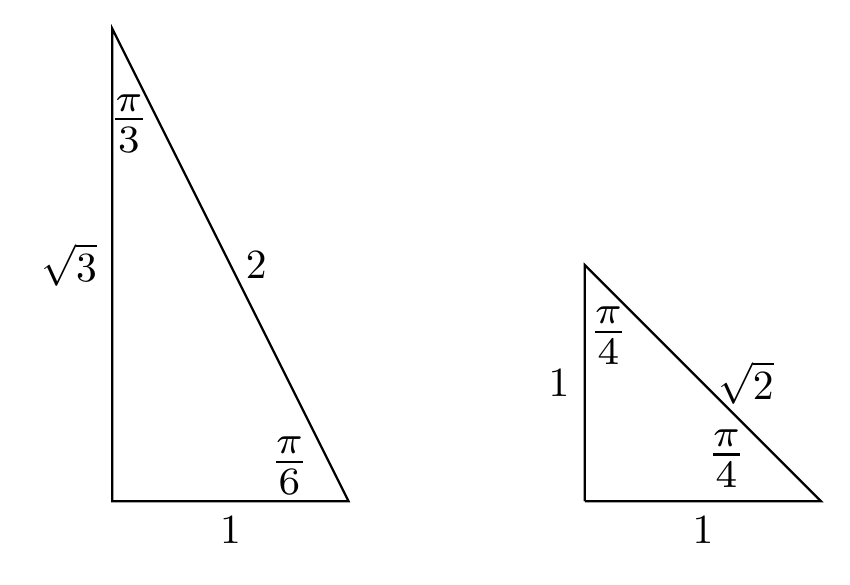
\begin{tikzpicture}[scale=3, thick, >=Stealth]
   \draw (0, 0) -- node[scale=1.5, below]{$1$} (1, 0)
                -- node[scale=1.5, right]{$2$} (0, 2)
                -- node[scale=1.5, left]{$\sqrt{3}$} cycle;
   \draw (0.75, 0.15) node[scale=2] {$\frac{\pi}{6}$};
   \draw (0.07, 1.6) node[scale=2] {$\frac{\pi}{3}$};

   \draw (2, 0) -- node[scale=1.5, left]{$1$} (2, 1)
                -- node[scale=1.5, right]{$\sqrt{2}$} (3, 0)
                -- node[scale=1.5, below]{$1$} (2,0);
   \draw (2.6, 0.18) node[scale=2] {$\frac{\pi}{4}$};
   \draw (2.1, 0.7) node[scale=2] {$\frac{\pi}{4}$};

\end{tikzpicture}
\end{document}
